\documentclass[bare_jrnl_transmag]{subfiles}
\begin{document}
\subsection{Drone Pose Estimation}
The drone pose estimation from the IMU is required to be accurate for the purposes of the VIO algorithm. Evaluation of the Madgwick filter was performed by comparing the ground-truth pose of the drone to the pose estimated by the Madgwick filter for a validation dataset. The results of the evaluation are shown in Figure \ref{fig:madgwick_results}.

\begin{figure}[H]
    \centering
    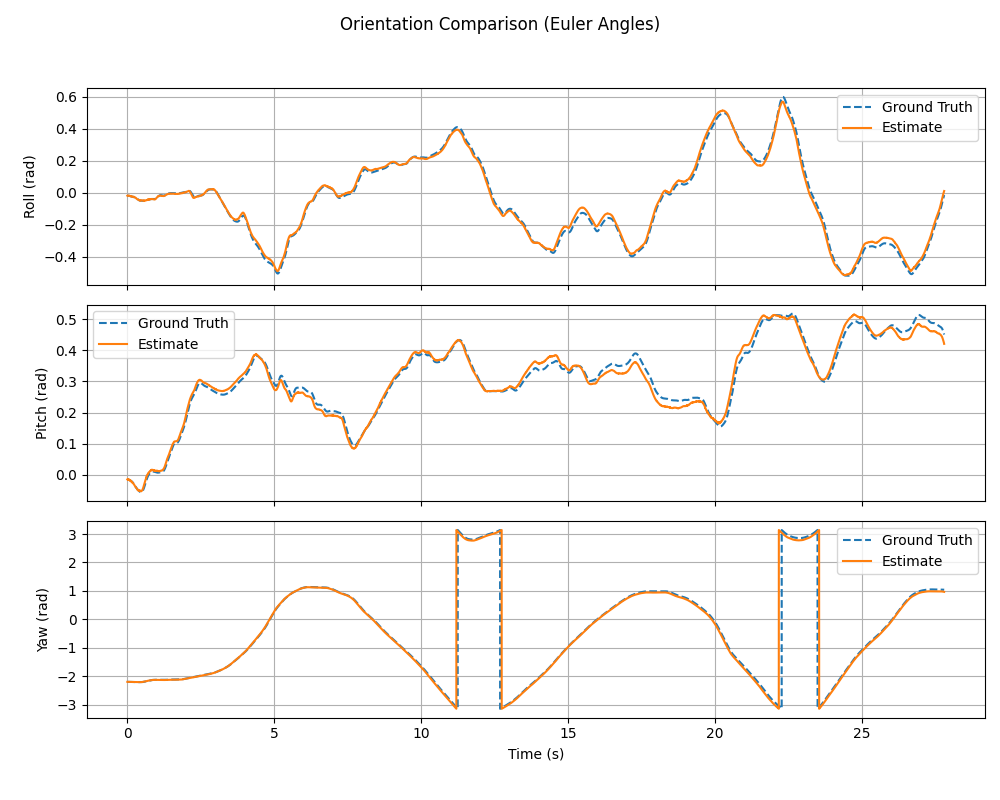
\includegraphics[width=0.8\linewidth]{figures/madgwick_results.png}
    \caption{Madgwick filter results. The blue line is the ground-truth pose of the drone, while the orange line is the pose angle estimated by the Madgwick filter.}
    \label{fig:madgwick_results}
\end{figure}

The results show that the Madgwick filter is able to estimate the pose of the drone with a high degree of accuracy (RMSE (Roll, Pitch, Yaw) - rad: [0.0198 0.0160 0.0425]) in real-time, making it suitable for use in the VIO algorithm.

A key limitation of the Madgwick filter is that it assumes the accelerometer measurements are only affected by gravity, and not by any other forces acting on the drone. This assumption is not valid in all cases, especially when the drone is moving quickly or performing aggressive maneuvers. When evaluating the filter's performance in high acceleration scenarios on the tuning dataset, the orientation estimation was found to diverge significantly and increase the RSME. Given the context of the dataset is an FPV drone where high acceleration maneuvers are common, the correction step size $\mu$ was made to be adaptive to the accelerometer measurements. The algorithm for the adaptive step size is shown in below, with the parameters $x_1$, $x_2$, and $x_3$ being tuned heuristically. This change helped improve the orientation estimation in high acceleration scenarios, though it does show some divergence in the presence of high acceleration noise. The algorithm is as follows:

\[
\mu_{\text{out}} =
\begin{cases}
0 & \text{if } \|\mathbf{a}\| \leq x_1 \\
\mu \cdot \dfrac{\|\mathbf{a}\| - x_1}{x_2 - x_1} & \text{if } x_1 < \|\mathbf{a}\| \leq x_2 \\
\mu \cdot \dfrac{x_3 - \|\mathbf{a}\|}{x_3 - x_2} & \text{if } x_2 < \|\mathbf{a}\| \leq x_3 \\
0 & \text{if } \|\mathbf{a}\| > x_3
\end{cases}
\]

\[
\text{where } x_1 = 4.905, \quad x_2 = 9.81, \quad x_3 = 14.715
\]



\end{document}